\documentclass[conference]{IEEEtran}
\usepackage{cite}
\usepackage{amsmath,amssymb,amsfonts}
\usepackage{algorithmic}
\usepackage{graphicx}
\usepackage{textcomp}
\usepackage{xcolor}
\usepackage{booktabs}
\usepackage{float}
\usepackage{pgf}

\title{Sum up Work on Intrusion Detection System in Vehicular Ad-hoc Networks}
\author{\IEEEauthorblockN{Johanes Wilian Ang}
\IEEEauthorblockA{\textit{Fakultas Teknologi Informasi} \\
\textit{Institut Teknologi Batam}\\
Batam, Indonesia \\
email: johanwilian455@gmail.com,}
}

\renewcommand{\IEEEkeywordsname}{Keywords}

\begin{document}

\maketitle
\begin{abstract}
    Deteksi intrusi dalam jaringan sangat pentinga karena sering terjadi serangan pada jaringan sehingga deteksi intrusi ini perlu diterapkan. Penyerang akan melakukan upaya untuk masuk ke sistem kita. Ada baiknya sistem kita terus dipantau dengan menggunakan intrusi untuk mendeteksi hal-hal yang mencurigakan, dan meresposnya ketika disusupi.
\end{abstract}

\section{pendahuluan}
    mendeteksi serangan lalu lintas jaringan, intrusi dan sebagainya.Saat ini, tantangan utama yang terkait dengan domain ini adalah untuk menjaga keamanan jaringan \cite {aydin2009hybrid}.
    
    sistem deteksi intrusi (IDS) Untuk mendeteksi intrusi di VANET, pembelajaran mesin, dan pembelajaran algoritma diberbagai tingkatan.
    
    susunan makalah disusun pada bab 2 akan menjelaskan tentang jaringan Ad-hoc. Bagian 3, menyajikan detail latar belakang dan membahas tentang teknologi berbeda yang terkait dengan pembelajaran mesin dan itu digunakan di VANET. Bagian 4 membahas tentang teknik logika fuzzy pada VANET

\section{Sistem Deteksi Intrusi}
    Komunikasi kendaraan memiliki tujuan utama untuk mendeteksi berbagai serangan lalu lintas dan mencegahnya dengan menggunakan Intrusion Detection System (IDS) tiga utama: komponen yang ditunjukkan pada Gambar 1 seperti pengumpulan data, vektorisasi dan mesin klasifikasi. IDS juga termasuk satu alasan utama untuk mendeteksi serangan kendaraan dari sistem, yang diketahui atau tidak diketahui. Umumnya IDS tergantung pada beberapa komponen perangkat keras. Menjalankan perangkat keras seperti itu komponen membutuhkan perangkat lunak yang konsisten dan kuat \cite {zhang2010research}.

\begin{center}
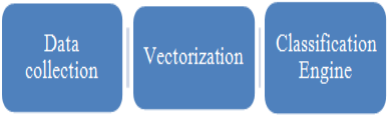
\includegraphics[width=.4\textwidth]{gambar/tugas7-1.PNG}

\end{center}

    alat komunikasi memiliki tujuan utama untuk mendeteksi berbagai serangan lalu lintas dan mencegahnya dengan menggunakan Intrusion Detection System (IDS),
    
    Mesin klasifikasi adalah bagian paling kompleks dari IDS karena termasuk keputusan vektor fitur yang dikonversi sebagai aturan penyusupan.
    
     IDS ini mengandung beberapa fakta, seperti:
     
     sistem komunikasi yang kompleks dan memiliki lebih banyak jumlah kesalahan.
     
     Mereka digunakan untuk mendeteksi kesalahan dan juga untuk memperbaikinya. Beberapa sistem pencegahan intrusi keluar tetapi tidak itu tidak akan mencegah semua serangan. Pada saat itu, IDS memainkan peran penting.
     
     Intrusion detection system is of two types: 1. Misuse based IDS 2. Anomaly based IDS.
     
     Jenis IDS berdasarkan deteksi serangan yang banyak diketahui telah ditentukan sebelumnya tetapi gagal untuk mengidentifikasi serangan yang tidak diketahui. Serangan tidak dikenal dengan alarm palsu tinggi dideteksi dengan menggunakan pendekatan berbasis anomali \cite{aydin2009hybrid}.
     
\section{Pekerjaan yang Berhubungan}
    Gozde Karatas et. Al.  \cite {karatas2018neural} mengusulkan Deteksi Intrusi Sistem [IDS] untuk menganalisis kinerja fungsi pelatihan dari sistem. Sistem yang diusulkan didasarkan pada sistem saraf jaringan yang berisi 2 lapisan tersembunyi untuk mendeteksi intrusi jaringan. Untuk analisis kinerja, Piala KDD 99 kumpulan data digunakan.
    
    Akash Garg et. Al. \cite {garg2016hybrid} mempresentasikan penggunaan berbasis penyalahgunaan atau IDS berbasis tanda tangan yang berfungsi saat data dikirim ke jaringan dan selanjutnya server memverifikasi data ini. Jika ada data kasar diperoleh, kemudian server membuang paket yang lain meneruskannya ke jaringan. Selanjutnya, data tiba di server diperiksa dengan menggunakan alat akurasi tinggi untuk mendeteksi paket jaringan dari database dan kemudian membuang paket jaringan lain itu akan memindahkan data ke sistem jaringan.
    
    Dalam \cite {gonccalves2019systematic}, disajikan studi tentang deteksi intrusi di VANET dan menganalisis solusi yang layak untuk berbagai jenis serangan seperti DOS, DDOS dll Tuan a Tang et. al \cite{tang2016deep} memberikan deskripsi terperinci tentang jaringan yang ditentukan perangkat lunak sebagai solusi yang dipilih untuk mendeteksi intrusi di jaringan. Penulis terutama berfokus pada serangan DDoS di IDS untuk meningkatkan akurasi model NIDS yang diusulkan dengan menggunakan teknik pembelajaran mendalam, yang mendeteksi intrusi dan menganalisis model NIDS.

    Konstantinos Pelechrinis et. Al. \cite {pelechrinis2010denial} menyajikan detail ulasan tentang serangan jamming yang direkam di koran oleh tambahan menjelaskan berbagai teknik yang disarankan untuk mendeteksi keberadaan jammer. Akhirnya, pekerjaan itu memiliki meninjau mekanisme yang banyak, yang bermanfaat untuk melindungi jaringan dari berbagai serangan jamming.
    
    Bellardo et al \cite {bellardo2003802}, mempresentasikan analisis eksperimental dari serangan tertentu dalam jaringan. Dalam penelitian ini diterapkan sistem untuk deteksi intrusi berdasarkan lapisan 802.11 MAC dan menganalisis efisiensi sistem
    
    Ismail Butun, dkk. Al. \cite {zhang2000intrusion} memberikan informasi tentang klasifikasi IDS, berisi klasifikasi rinci pf sistem deteksi intrusi sebagai persyaratan IDS, klasifikasi, pengambilan keputusan di IDS dan intrusi tanggapan. IDS yang diusulkan untuk Mobile Ah-hoc NETworks (MANET) disajikan dan penerapannya untuk jaringan sensor nirkabel dibahas.
    
\section{Kategori Serangan}
Serangan lalu lintas dalam sistem komunikasi adalah
berbeda sebagai berikut:

\begin{itemize}
    \item normal
    \item DOS
    \item U2R
    \item R2L
    \item Probe
\end{itemize}

Serangannya terdiri dari 22 jenis, masing-masing milik serangan
kategori di atas \cite {butun2013survey}.

\textbf{DOS}: Sebuah upaya untuk membuat layanan
tidak tersedia untuk pengguna dikenal sebagai DoS (Denial of Service). Di
serangan ini, tujuan penyerang adalah agar node tidak dapat melakukan yang lain
tugas yang perlu dan esensial. Ini yang paling parah dan
serangan yang kompleks sama sekali. Serangan ini dapat membebani sumber daya
node jaringan dengan mengganggu saluran dengan cara jaringan.
Ini adalah serangan lapisan fisik yang mengandung sub-tipe DDoS
(Penolakan Serangan Terdistribusi).

\textbf{U2R}: Serangan utama pada pengguna untuk melakukan root
(U2R) adalah buffer overflow yang menyalin terlalu banyak data ke dalam
buffer statis tanpa memeriksa apakah sudah diperbaiki dengan benar atau tidak.

\textbf{R2L}: Serangan ini mempengaruhi besar jumlah jaringan/sistem di dunia setiap hari.

\textbf{Probe}: Attacker tries to gain information about 
the target host.

\section{Teknik Machine Learning}
Untuk mendeteksi intrusi dalam komunikasi kendaraan beberapa
pembelajaran mesin dan algoritma pembelajaran mendalam digunakan.
Beberapa algoritma ditinjau di sini di bawah ini juga:

Deep Belief Network (DBN): Jaringan Kepercayaan Dalam
memiliki jaringan saraf umpan maju dengan kedalaman
arsitektur terdiri dari banyak lapisan tersembunyi. Beberapa terlihat
lapisan disebut sebagai lapisan input dan juga beberapa lapisan output adalah
menyajikan. Dalam \cite{olusola2010analysis} digunakan protokol routing cerdas berbasis based
jaringan kepercayaan yang mendalam untuk layanan multimedia dalam pengetahuan
VANET sentris. DBN melakukan deteksi intrusi
melalui berbagai eksperimen setelah pelatihan dengan beberapa
kumpulan data juga meningkatkan jaringan keamanan dengan standar
algoritma IDS. DBN sebagian besar jatuh sekarang dan
jarang digunakan dibandingkan dengan algoritma pembelajaran generatif lainnya
tetapi masih diakui untuk peran penting mereka dalam pembelajaran yang mendalam.

Algoritma K-Means: Algoritma K-mean dapat digunakan
untuk mengembangkan sistem deteksi intrusi. [12]\cite{zhang2018intelligent} Algoritma ini
tidak menentukan jumlah cluster dan cluster adalah
dibuat menggunakan nilai optimal berdasarkan fungsi fitness untuk
membantu mengidentifikasi jenis serangan.

Support Vector Machine (SVM): In \cite{sukumar2018network} implemented 
SVM against network intrusion using MATLAB. KDD 
dataset is used as bench market dataset for intrusion 
detection and shows SVM is limited because they need long 
training time to show the result. 

Convolutional Neural Network (CNN): CNN sangat dalam
algoritma pembelajaran yang digunakan untuk mengklasifikasikan gambar dan mengenali
yang benar dengan akurasi tinggi. Model ini terdiri dari
neuron dengan data yang dapat dipelajari yang dilewatkan dari berbagai lapisan
seperti lapisan yang sepenuhnya terhubung, penyatuan, filter, dan fungsi. Di
\cite{lahre2013analyze} memberikan perbandingan deep learning CNN dengan DBN.
Menurut hasil kinerja CNN menunjukkan bahwa
akurasi dan deteksi model CNN dalam intrusi
deteksi sedikit lebih tinggi dari model DBN.

Memori jangka pendek panjang (LSTM): Jangka pendek panjang
jaringan memori adalah jaringan saraf berulang yang mampu
urutan pembelajaran dalam urutan masalah prediksi. LSTM adalah
area pembelajaran mendalam yang kompleks. Supriya P. Shende et. Al. \cite{yong2019intrusion}
menyimpulkan bahwa biner serta klasifikasi multiclass
untuk deteksi menggunakan LSTM dalam keamanan jaringan. Berdasarkan
akurasi penulis LSTM dalam keamanan jaringan pembelajaran mendalam
untuk biner 99,2 persen

\section{Penggunan Data Set}
Kumpulan data yang paling umum digunakan untuk deteksi intrusi
di IDS adalah: KDD Cup99, NSL-KDD, CIC IDS 2017, CSE CIC-IDS 2018

\textbf{KDD Cup99}: Dataset KDD Cup99 dibuat pada tahun 1999
untuk mendeteksi intrusi. Dataset digunakan dalam penambangan data dan
teknik pembelajaran mesin. Dataset ini berisi sekitar 4.9
juta keping data, di mana 83% di antaranya diklasifikasikan untuk semua
jenis serangan.

\textbf{NSL-KDD:}Algoritme pembelajaran mesin pada KDD Cup99 dapat melakukan pra-proses dengan baik dan membuat kumpulan data KDD NSL baru dengan menghapus catatan duplikat darinya. Begitu
sebelumnya, banyak perbedaan telah ditemukan di yang baru
kumpulan data dibandingkan dengan kumpulan data lama


\textbf{CIC IDS 2017:} Dataset ini mencakup serangan umum seperti
data dunia nyata, menggabungkan berbagai kriteria untuk mengidentifikasi serangan serta memberikan hasil yang tepat untuk pembelajaran mesin
dan pembelajaran yang mendalam.

\textbf{CS E-CIC-IDS 2018:}Untuk sistem kendaraan, detail
informasi serangan disertakan di dalamnya. Kumpulan data ini berisi:
tujuh jenis serangan beberapa terkait dengan kendaraan
komunikasi seperti serangan DoS, serangan DDOS, Brute
serangan paksa, dll.

\section{Arsitektur yang DiUsulkan}

\begin{center}
    \centering
    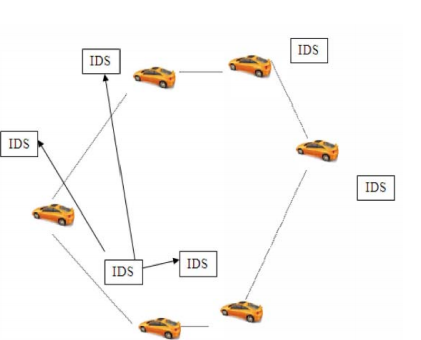
\includegraphics[width=.4\textwidth]{gambar/tugas7-2.PNG}
    \end{center}
    Gambar 2. Kerangka kerja Sistem Deteksi Intrusi di VANET
    Sistem deteksi intrusi yang diusulkan dapat mendeteksi
    intrusi menggunakan data audit jika ada perubahan data. Ini
    melibatkan beberapa perilaku umum untuk deteksi intrusi
    node. Data audit yang dikumpulkan terhadap intrusi diperiksa.
    \begin{center}
        \centering
        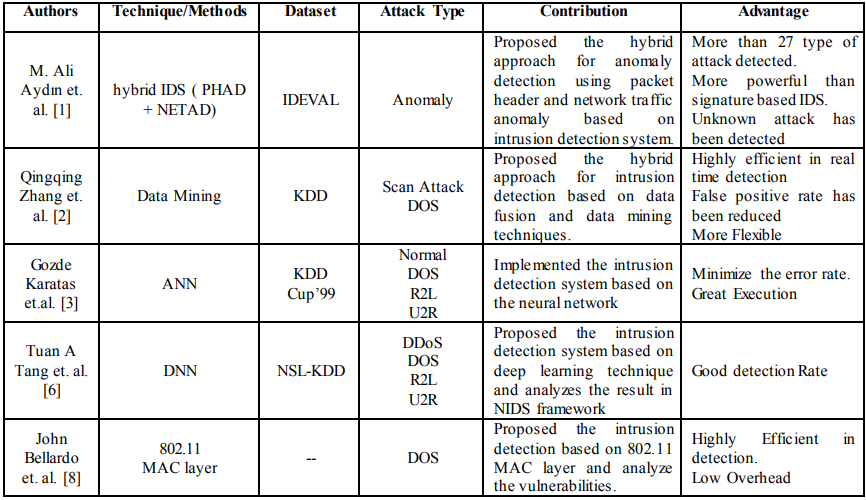
\includegraphics[width=.4\textwidth]{gambar/a.PNG}
        \end{center}
        \begin{center}
        \centering
        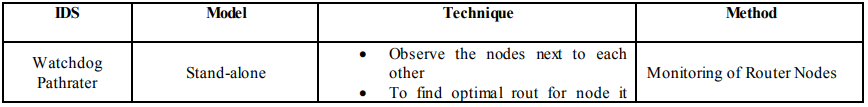
\includegraphics[width=.4\textwidth]{gambar/b.PNG}
        \end{center}
        \begin{center}
        \centering
        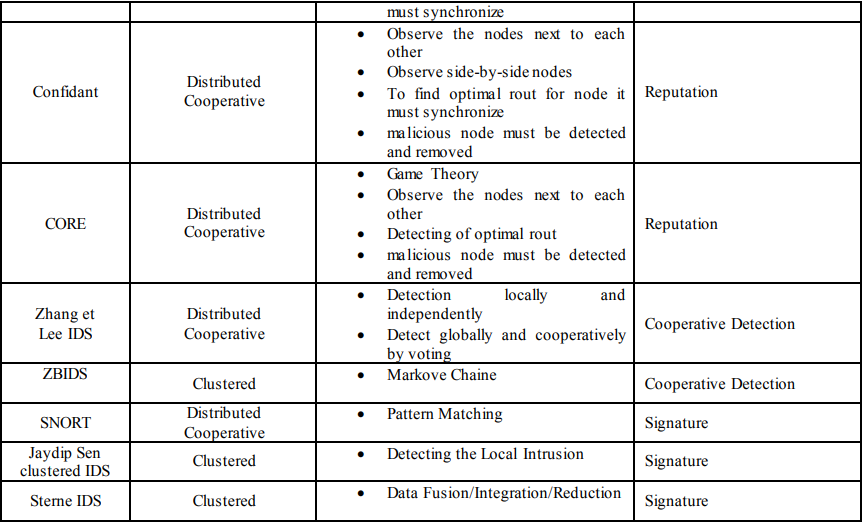
\includegraphics[width=.4\textwidth]{gambar/c.PNG}
        \end{center}
        
Operasi jaringan kendaraan harus menyediakan setiap node dengan
teknik deteksi intrusi sehingga setiap node dapat
berpartisipasi dalam deteksi intrusi. Node tetangga bisa
membentuk asosiasi dan mengawasi jaringan satu sama lain.
VANET berisi agen untuk mendeteksi intrusi setiap node
dan agen-agen ini bertindak secara independen dan mengendalikan
kegiatan komunikasi dalam jangkauan radio. Jika ada
perubahan data lokal, agen dari node tetangga akan
membantu mendeteksi penyusupan.

\section{Diskusi}
Dalam mempelajari teknik deteksi intrusi yang berbeda
diusulkan dalam penelitian sebelumnya dan akhirnya menyimpulkan bahwa
sebagian besar sistem deteksi intrusi yang ada telah
terdistribusi dan didasarkan pada berbagai jenis anomali
deteksi. Dalam mempelajari deteksi intrusi yang berbeda
teknik yang diusulkan dalam penelitian sebelumnya dan akhirnya
menyimpulkan bahwa sebagian besar deteksi intrusi yang ada
sistem telah didistribusikan dan didasarkan pada berbagai
jenis deteksi anomali. Selain itu, pembelajaran mesin
teknik telah digunakan untuk mendeteksi intrusi seperti ini:
teknik pembelajaran mesin lebih efisien mengatasi
pencarian dan analisis masalah dengan berbagai macam sumber daya.

\section{Kesimpulan}
VANET sangat rentan terhadap serangan karena nirkabel
media dan kurangnya fitur keamanan tradisional. Keamanan
harus menjadi prioritas utama bagi pengguna jalan. Jadi keamanan
aplikasi perlu bekerja pada hal-hal seperti notifikasi
sebelum terjadi kecelakaan. Dalam makalah ini kita telah membahas
berbagai jenis serangan intrusi dan ditinjau
studi yang ada. Menunjukkan apakah jaringan tersedia
untuk komunikasi yang aman. Studi ini menemukan bahwa sebagian besar
kumpulan data tidak mengenali atau memberi tahu bagaimana konten dan serangan
diciptakan. Selain itu, pembuat kumpulan data tidak membuat
kumpulan data tersedia untuk umum untuk ditinjau. Deteksi gangguan
sistem dapat menciptakan teknik pencegahan untuk memperkuat
keamanan jaringan.

Di masa depan, tujuannya adalah untuk merancang kerangka kerja untuk intrusi
deteksi di VANET. Tujuan utama dari penelitian ini adalah untukbuat kumpulan data besar untuk membuat pembelajaran mesin
algoritma lebih efisien. Semua kriteria ini harus
dipertimbangkan untuk membuat kumpulan data yang besar, mengidentifikasi
menyerang, dan membuat pesan.

\bibliographystyle{IEEEtran}
\bibliography{referensi.bib}

\end{document}
